\chapter{Zeitenkontrolle}
Für die Zeitenkontrolle wurden die Daten aus Jira ausgewertet und im folgenden Abschnitt analysiert.

\section{Zeitaufwand pro Person }
\begin{figure}[H]
	\centering
	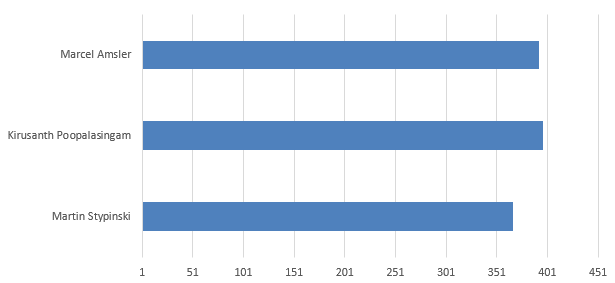
\includegraphics[width=1.0\textwidth] {images/time-per-person.png}
	\caption{Zeitaufwand pro Person in Stunden}
	\label{fig:time}
\end{figure}

Die gezeigte Grafik \ref{fig:time} zeigt total aufgewendeten Stunden während dem Projekt. Es wurden leicht mehr Stunden investiert, als die geforderten 360, welche 12 ECTS Punkten entsprechen. Um am Ende des Projekts einen Stand zu haben, der auch als Plattform veröffentlicht werden kann, wurde im Team beschlossen die zusätzliche Zeit zu investieren.

\section{Zeitaufwand nach Task}
\begin{figure}[H]
	\centering
	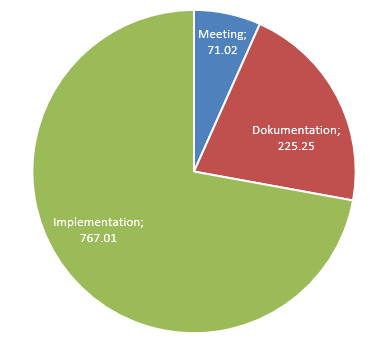
\includegraphics[width=0.6\textwidth] {images/time-per-category.png}
	\caption{Zeitaufwand pro Kategorie}
	\label{fig:time-per-category}
\end{figure}

Wie aus der Grafik \ref{fig:time-per-category} zu entnehmen ist, wurde für die Implementierung die meiste Zeit aufgewendet. Das Testing gehört zur Implementation (siehe Kapitel \ref{quality-assurance} Qualitätssicherung ) und wurde nicht separat geführt. Die Kategorie Meetings beinhaltet die Treffen mit dem Betreuer, Team-interne Meetings und die Zwischenpräsentation.

